% Options for packages loaded elsewhere
\PassOptionsToPackage{unicode}{hyperref}
\PassOptionsToPackage{hyphens}{url}
\documentclass[
  10pt,
  a4paper,
]{article}
\usepackage{xcolor}
\usepackage[margin=22mm]{geometry}
\usepackage{amsmath,amssymb}
\setcounter{secnumdepth}{-\maxdimen} % remove section numbering
\usepackage{iftex}
\ifPDFTeX
  \usepackage[T1]{fontenc}
  \usepackage[utf8]{inputenc}
  \usepackage{textcomp} % provide euro and other symbols
\else % if luatex or xetex
  \usepackage{unicode-math} % this also loads fontspec
  \defaultfontfeatures{Scale=MatchLowercase}
  \defaultfontfeatures[\rmfamily]{Ligatures=TeX,Scale=1}
\fi
\usepackage{lmodern}
\ifPDFTeX\else
  % xetex/luatex font selection
\fi
% Use upquote if available, for straight quotes in verbatim environments
\IfFileExists{upquote.sty}{\usepackage{upquote}}{}
\IfFileExists{microtype.sty}{% use microtype if available
  \usepackage[]{microtype}
  \UseMicrotypeSet[protrusion]{basicmath} % disable protrusion for tt fonts
}{}
\makeatletter
\@ifundefined{KOMAClassName}{% if non-KOMA class
  \IfFileExists{parskip.sty}{%
    \usepackage{parskip}
  }{% else
    \setlength{\parindent}{0pt}
    \setlength{\parskip}{6pt plus 2pt minus 1pt}}
}{% if KOMA class
  \KOMAoptions{parskip=half}}
\makeatother
\usepackage{graphicx}
\makeatletter
\newsavebox\pandoc@box
\newcommand*\pandocbounded[1]{% scales image to fit in text height/width
  \sbox\pandoc@box{#1}%
  \Gscale@div\@tempa{\textheight}{\dimexpr\ht\pandoc@box+\dp\pandoc@box\relax}%
  \Gscale@div\@tempb{\linewidth}{\wd\pandoc@box}%
  \ifdim\@tempb\p@<\@tempa\p@\let\@tempa\@tempb\fi% select the smaller of both
  \ifdim\@tempa\p@<\p@\scalebox{\@tempa}{\usebox\pandoc@box}%
  \else\usebox{\pandoc@box}%
  \fi%
}
% Set default figure placement to htbp
\def\fps@figure{htbp}
\makeatother
\setlength{\emergencystretch}{3em} % prevent overfull lines
\providecommand{\tightlist}{%
  \setlength{\itemsep}{0pt}\setlength{\parskip}{0pt}}
\usepackage{mathrsfs}
\newcommand{\Log}{\operatorname{Log}}
\usepackage{mathtools}
\usepackage{xurl}
\emergencystretch=3em
\setcounter{tocdepth}{1}
\newcommand{\Beta}{\mathrm{B}}
\DeclareUnicodeCharacter{00B2}{\ensuremath{^2}}
\DeclareUnicodeCharacter{00B1}{\ensuremath{\pm}}
\DeclareUnicodeCharacter{00D7}{\ensuremath{\times}}
\DeclareUnicodeCharacter{2192}{\ensuremath{\to}}
\DeclareUnicodeCharacter{21D2}{\ensuremath{\Rightarrow}}
\DeclareUnicodeCharacter{21A6}{\ensuremath{\mapsto}}
\DeclareUnicodeCharacter{2208}{\ensuremath{\in}}
\DeclareUnicodeCharacter{2209}{\ensuremath{\notin}}
\DeclareUnicodeCharacter{2212}{\ensuremath{-}}
\DeclareUnicodeCharacter{2227}{\ensuremath{\wedge}}
\DeclareUnicodeCharacter{2228}{\ensuremath{\vee}}
\DeclareUnicodeCharacter{2260}{\ensuremath{\ne}}
\DeclareUnicodeCharacter{2264}{\ensuremath{\le}}
\DeclareUnicodeCharacter{2265}{\ensuremath{\ge}}
\DeclareUnicodeCharacter{2297}{\ensuremath{\otimes}}
\DeclareUnicodeCharacter{00B3}{\ensuremath{^3}}
\DeclareUnicodeCharacter{2074}{\ensuremath{^4}}
\DeclareUnicodeCharacter{2076}{\ensuremath{^6}}
\DeclareUnicodeCharacter{03BB}{\ensuremath{\lambda}}
\DeclareUnicodeCharacter{03BC}{\ensuremath{\mu}}
\DeclareUnicodeCharacter{03B5}{\ensuremath{\epsilon}}
\DeclareUnicodeCharacter{03C4}{\ensuremath{\tau}}
\DeclareUnicodeCharacter{03A6}{\ensuremath{\Phi}}
\DeclareUnicodeCharacter{03B1}{\ensuremath{\alpha}}
\DeclareUnicodeCharacter{03C3}{\ensuremath{\sigma}}
\DeclareUnicodeCharacter{03B4}{\ensuremath{\delta}}
\DeclareUnicodeCharacter{03C0}{\ensuremath{\pi}}
\DeclareUnicodeCharacter{039B}{\ensuremath{\Lambda}}
\DeclareUnicodeCharacter{2202}{\ensuremath{\partial}}
\DeclareUnicodeCharacter{0393}{\ensuremath{\Gamma}}
\DeclareUnicodeCharacter{2205}{\ensuremath{\varnothing}}
\DeclareUnicodeCharacter{221E}{\ensuremath{\infty}}
\DeclareUnicodeCharacter{2200}{\ensuremath{\forall}}
\DeclareUnicodeCharacter{00B9}{\ensuremath{^1}}
\DeclareUnicodeCharacter{00B0}{\ensuremath{{}^\circ}}
\DeclareUnicodeCharacter{211D}{\ensuremath{\mathbb{R}}}
\usepackage{bookmark}
\IfFileExists{xurl.sty}{\usepackage{xurl}}{} % add URL line breaks if available
\urlstyle{same}
\hypersetup{
  hidelinks,
  pdfcreator={LaTeX via pandoc}}

\author{}
\date{}

\begin{document}

{
\setcounter{tocdepth}{3}
\tableofcontents
}
\section{The escaping inverse fibre, its infinitesimal boundary, and its
trace
form}\label{the-escaping-inverse-fibre-its-infinitesimal-boundary-and-its-trace-form}

This derivation retains the original polynomial map, its target
coordinates, and its heat constants. It computes an actual dual-number
fibre at every double collision, the larger boundary at a triple
collision, the exact maps under which infinitesimals vanish, and the
signatures of the associated finite trace forms. It does not identify
these finite trace forms with the classical Weil distribution. No
off-critical zero of the Riemann zeta function is asserted.

\subsection{Sources actually read}\label{sources-actually-read}

The complete original LaTeX files
\texttt{tex/\allowbreak{}satellites/\allowbreak{}26\_\allowbreak{}incompressible\_\allowbreak{}fibre\_\allowbreak{}heat.\allowbreak{}tex} and
\texttt{tex/\allowbreak{}satellites/\allowbreak{}23\_\allowbreak{}source\_\allowbreak{}mechanism\_\allowbreak{}transfer.\allowbreak{}tex} in the local
\texttt{Zeta-\allowbreak{}Function-\allowbreak{}Foundation} repository were read for this
calculation. The received source formulas are \texttt{eq:\allowbreak{}ifh-\allowbreak{}original},
\texttt{eq:\allowbreak{}ifh-\allowbreak{}det}, \texttt{eq:\allowbreak{}ifh-\allowbreak{}chart},
\texttt{eq:\allowbreak{}ifh-\allowbreak{}target-\allowbreak{}chart}, \texttt{eq:\allowbreak{}ifh-\allowbreak{}target-\allowbreak{}flow},
\texttt{eq:\allowbreak{}ifh-\allowbreak{}triple}, \texttt{eq:\allowbreak{}retained-\allowbreak{}node-\allowbreak{}map}, and
\texttt{eq:\allowbreak{}retained-\allowbreak{}arithmetic-\allowbreak{}extension}. Their original-map provenance
is
\href{https://terrytao.wordpress.com/2026/07/21/a-digestion-of-the-jacobian-conjecture-counterexample/}{Tao's
displayed map and explanation} and
\href{https://sbseminar.wordpress.com/2026/07/20/the-new-counterexample-to-the-jacobian-conjecture/}{Speyer's
marked-factor discussion}, as cited in those programme sources. The
full-support definition used below is reproduced in FSR1--FSR7 of
\href{https://github.com/KokunoYumeto/zeta-function-research-reader/blob/173dbc6ed5a03235dbe7654f928f3692107db39b/workbenches/splitzero-tandem/branches/tau-zero-prime-positivity/FULL_SUPPORT_RECONSTRUCTION_DERIVATION.md}{full-support
reconstruction proof}; its first 70 lines were read. The results below
supply their own algebraic proofs.

The exact read coverage was lines 1--480 of the first file, SHA256
\texttt{72058517\allowbreak{}553FF3A2\allowbreak{}C3569984\allowbreak{}4FA95BBA\allowbreak{}9EC695E7\allowbreak{}74E0E3D4\allowbreak{}CF33CF7B\allowbreak{}84DA51DD},
and lines 1--666 of the second file, SHA256
\texttt{D8A65C46\allowbreak{}B78A5ACE\allowbreak{}521A164A\allowbreak{}ABC99F24\allowbreak{}6908058E\allowbreak{}36B60C35\allowbreak{}BCE938D5\allowbreak{}1C020898}.
These are local programme source versions, not author-source archives.

The forward heat time called tau in the source is denoted \(h\) here,
solely to keep it distinct from the global absorber \(\tau_L\). The
displacement from a specified collision is \(d=h-h_c\). All original
spatial and target coordinates are retained.

\subsection{1. Original map and projective inverse
chart}\label{original-map-and-projective-inverse-chart}

Over \(\mathbb C\), write \[
\begin{aligned}
F_1&=(1+xy)^3w+y^2(1+xy)(4+3xy),\\
F_2&=y+3x(1+xy)^2w+3xy^2(4+3xy),\\
F_3&=2x-3x^2y-x^3w.
\end{aligned}
\tag{EFI1}
\] The target is \((a,b,c)\). Define \[
P(r)=cr^3-2r^2+br-2a,\qquad
\alpha=\frac{P'(r)}2,\qquad
H(r,\alpha,c)=\left(\frac1\alpha,r-\alpha,
5\alpha^2-3r\alpha-c\alpha^3\right).
\tag{EFI2}
\] Direct substitution before imposing \(P=0\) gives \[
F\circ H=(r^2+r\alpha-cr^3,\ 4r+2\alpha-3cr^2,\ c).
\tag{EFI3}
\] Consequently \(F_2=b\) is exactly \(2\alpha=P'(r)\), and then
\(2(F_1-a)=P(r)\). Conversely, from a finite point with \(x\ne0\),
recover \(\alpha=1/x\) and \(r=y+1/x\); solving \(F_3=c\) recovers every
coordinate of EFI2. This proves that simple roots of \(P\) are in
bijection with all inverse points with \(x\ne0\). No multiple root
supplies a finite point in this chart. On the excluded hyperplane, \[
F(0,y,w)=(w+4y^2,y,0).
\tag{EFI4}
\] Thus a separate finite point \((0,b,a-4b^2)\) exists exactly when
\(c=0\).

Put projective coordinates \([X:Y:W:T]\) on the compactification of the
source, with affine coordinates \((x,y,w)=(X/T,Y/T,W/T)\). Multiplying
the homogeneous representative of EFI2 by \(\alpha\) gives the
everywhere defined map \[
\overline H(r,\alpha,c)=
[1:\alpha(r-\alpha):5\alpha^3-3r\alpha^2-c\alpha^4:\alpha].
\tag{EFI5}
\] It agrees with the actual inverse point when \(\alpha\ne0\). Every
point with \(\alpha=0\) maps to \[
p_\infty=[1:0:0:0].
\tag{EFI6}
\] This equality of projective points does not identify their
infinitesimal neighbourhoods. Those neighbourhoods are computed below.

\subsection{2. The original two escaping trajectories give exact dual
numbers}\label{the-original-two-escaping-trajectories-give-exact-dual-numbers}

On the original target line \(b=c=0\), the entire root cover is \[
a=-r^2,\qquad \alpha=-2r,
\qquad (x,y,w)=\left(-\frac1{2r},3r,26r^2\right)\quad(r\ne0).
\tag{EFI7}
\] These equalities follow by substituting \(c=b=0\) in EFI2. In
particular, the projective graph is \[
(r,a)\longmapsto
\bigl([1:-6r^2:-52r^3:-2r],\ a=-r^2\bigr).
\tag{EFI8}
\] In the projective chart \(X=1\), its coordinate \(T/X=-2r\) recovers
\(r\). Hence this map identifies the graph closure with the affine
\(r\)-line; its completed local ring at the escaping point is
\(\mathbb C[[r]]\). The base parameter map is exactly \[
\mathbb C[[a]]\longrightarrow\mathbb C[[r]],\qquad a\longmapsto-r^2.
\tag{EFI9}
\] The scheme fibre over \(a=0\) is therefore \[
\mathbb C[[r]]/(a)=\mathbb C[r]/(r^2)
\xrightarrow[\sim]{r\mapsto\epsilon}
D:=\mathbb C[\epsilon]/(\epsilon^2).
\tag{EFI10}
\] The inverse is \(\epsilon\mapsto r\). The class \(r\) is nonzero
because the two residue classes \(1,r\) are linearly independent. Thus
dual numbers arise from the special fibre of the actual inverse map;
they have not been introduced by a resemblance of notation.

The additional finite point of EFI4 is \((0,0,a)\) and survives at
\(a=0\). It is a different component of the compactified inverse fibre.
The length-two point EFI10 is supported at infinity, while this extra
point is supported at the finite origin. Keeping both preserves total
fibre length three on this line.

The original forward heat orbit has \[
a=-\frac14+2h,\qquad r^2=\frac14-2h,
\qquad d=h-\frac18,\qquad r^2=-2d.
\tag{EFI11}
\] For \(h<1/8\), taking \(r=\mp\sqrt{1-8h}/2\) in EFI7 recovers exactly
\[
\gamma_\pm(h)=
\left(\pm(1-8h)^{-1/2},
\mp\frac32(1-8h)^{1/2},\frac{13}2(1-8h)\right).
\tag{EFI12}
\] Thus the dual-number boundary is attached to those same escaping
trajectories with the same time constant.

\subsubsection{The exact cancellation and the retained
tangent}\label{the-exact-cancellation-and-the-retained-tangent}

For a holomorphic germ \(f(r)=\sum_{n\ge0}f_nr^n\) on the graph, the
sheet involution is \(\sigma(r)=-r\). The trace is \[
\operatorname{Tr}(f)=f(r)+f(-r)=2\sum_{n\ge0}f_{2n}r^{2n}.
\tag{EFI13}
\] This is a map to \(\mathbb C[[a]]\) under EFI9. Its kernel is exactly
\(r\mathbb C[[a]]\), and the trace divided by two has the even-section
inclusion as a right inverse. This proves exactly what the sheet trace
forgets.

The antisymmetric functional satisfies \[
\frac{f(r)-f(-r)}{2r}\longrightarrow f_1=f'(0)
\quad\text{as }r\longrightarrow0.
\tag{EFI14}
\] The equality follows directly from its power series, which equals
\(f_1+f_3r^2+f_5r^4+\cdots\). On a germ pulled back from \(a=-r^2\), the
numerator is identically zero. On the projective coordinate \(T/X=-2r\),
the limit is \(-2\). Therefore the retained limit is a nonzero tangent
functional at \(p_\infty\), killed by projection to the target. Its
algebra map is precisely EFI10.

This limit does not assign a finite value to the pole \(x=-1/(2r)\).
Indeed the two sheet sums and the quadratic moment are \[
x(r)+x(-r)=0,
\qquad x(r)-x(-r)=-\frac1r,
\qquad x(r)^2+x(-r)^2=\frac1{2r^2}=-\frac1{2a}.
\tag{EFI15}
\] Thus a first-moment cancellation coexists with a divergent second
moment. The latter is the explicit retained defect in any proposed
assertion that all observables cancel.

\subsection{3. Every double collision in the given heat
family}\label{every-double-collision-in-the-given-heat-family}

Fix a double root \(r_0\) at a target \((a_0,b_0,c_0)\). Put \[
q_0=3c_0r_0-2\ne0,\qquad t=r-r_0,
\qquad a=a_0+2d,\quad b=b_0+6c_0d,\quad c=c_0.
\tag{EFI16}
\] The inequality \(q_0\ne0\) says exactly that the root has
multiplicity two rather than three, since \(P''(r_0)=2q_0\). Taylor
expansion of this cubic is an exact identity, with no omitted remainder:
\[
P=q_0t^2+c_0t^3+2q_0d+6c_0dt.
\tag{EFI17}
\] In the completed local ring at \((d,t)=(0,0)\), the factor
\(2q_0+6c_0t\) is a unit. Hence EFI17 is equivalent to \[
d=-\frac{t^2(q_0+c_0t)}{2q_0+6c_0t},
\qquad
\alpha=q_0t+\frac32c_0t^2+3c_0d.
\tag{EFI18}
\] The completed root ring is \(\mathbb C[[t]]\) with exactly this base
map. The coefficient of \(t\) in \(\alpha\) is \(q_0\ne0\). A formal
series with a nonzero linear coefficient has a unique inverse series:
its coefficient of degree one is determined by division by \(q_0\), and
at every later degree the new unknown enters multiplied by the same
nonzero \(q_0\). This recursive argument proves
\(\mathbb C[[\alpha]]=\mathbb C[[t]]\).

Since \(T/X=\alpha\) is a coordinate of the projective graph, the graph
completion is this same ring. In EFI18 the coefficient multiplying
\(t^2\) is a unit, so the special fibre is \[
\mathbb C[[t]]/(d)=\mathbb C[t]/(t^2).
\tag{EFI19}
\] The projective tangent has \[
T/X=q_0t,\qquad Y/X=r_0q_0t,\qquad W/X=0
\quad\text{modulo }t^2.
\tag{EFI20}
\] This retains the original constants and the actual tangent direction.
For \(c_0=0\), one has \(q_0=-2\), and EFI18 gives exactly \(d=-t^2/2\),
including the quadratic calculation above.

\subsection{4. Triple collision: root fibre and projective graph fibre
differ by exact
maps}\label{triple-collision-root-fibre-and-projective-graph-fibre-differ-by-exact-maps}

Now fix \(c\ne0\) and the triple target \[
r_* =\frac{2}{3c},\qquad
a_* =\frac{4}{27c^2},\qquad b_* =\frac4{3c}.
\tag{EFI21}
\] Along its heat orbit \(a=a_*+2d, b=b_*+6cd\), put \(z=r-r_*\). The
exact equations are \[
P=c(z^3+6dz),\qquad
\alpha=\frac{3c}{2}z^2+3cd.
\tag{EFI22}
\] Let \(R=\mathbb C[d]\) and \[
B=R[z]/(z^3+6dz).
\tag{EFI23}
\] It is free of rank three over \(R\), with ordered basis \(1,z,z^2\),
by division by the displayed monic cubic. Its completed local ring is
\(\widehat B=\mathbb C[[d,z]]/(z^3+6dz)\). Its special root fibre is \[
B_0=B/(d)=\mathbb C[z]/(z^3).
\tag{EFI24}
\] This is a length-three infinitesimal, rather than a length-two one.
It has the surjection \(B_0\to D, z\mapsto\epsilon\), with kernel
\((z^2)\). It also contains the subalgebra \(\mathbb C[z^2]\cong D\),
with \(\epsilon\mapsto z^2\). There is no retraction of this latter
inclusion: any homomorphism \(B_0\to D\) sends \(z\) to a nilpotent
multiple of \(\epsilon\), whose square is zero, whereas a retraction
would have to send \(z^2\) to \(\epsilon\ne0\).

\subsubsection{The graph closure itself}\label{the-graph-closure-itself}

In the projective chart \(X=1\), write \[
\eta=Y/X=\alpha(r_*+z-\alpha),\qquad
\omega=W/X=5\alpha^3-3(r_*+z)\alpha^2-c\alpha^4.
\tag{EFI25}
\] The projective graph algebra is the \(R\)-subalgebra
\(A=R[\alpha,\eta,\omega]\subset B\). Define \[
u=z^2=\frac{2}{3c}(\alpha-3cd),
\qquad
v=dz=-\frac{\eta-r_*\alpha+\alpha^2}{6c}.
\tag{EFI26}
\] The second equality follows because
\(\alpha z=(3c/2)z^3+3cdz=-6cdz\). Thus \(u,v\in A\). Conversely
\(\alpha=(3c/2)u+3cd\), \(\eta=r_*\alpha-\alpha^2-6cv\), and \[
\omega=5\alpha^3-3r_*\alpha^2+18c\alpha v-c\alpha^4.
\tag{EFI27}
\] All projective coordinates therefore belong to \(R[u,v]\), proving
\(A=R[u,v]\) inside \(B\).

Products in this ring satisfy exactly \[
u^2=-6du,\qquad uv=-6dv,\qquad v^2=d^2u.
\tag{EFI28}
\] For example \(u^2=z^4=-6dz^2\), and the other identities follow in
the same manner. Every word in \(u,v\) reduces, by these identities, to
an \(R\)-linear combination of \(1,u,v\). These three elements are
linearly independent in \(B\): a relation would have coefficients
\(A_0+A_1z^2+A_2dz=0\), and the basis \(1,z,z^2\) forces
\(A_0=A_1=dA_2=0\); the polynomial ring \(R\) has no \(d\)-torsion.
Hence \[
A\cong
R[u,v]/(u^2+6du,\ uv+6dv,\ v^2-d^2u),
\qquad A=R\oplus Ru\oplus Rv.
\tag{EFI29}
\] This proves that the displayed relations are complete.

For \(d\ne0\), \(z=v/d\), so \(A[d^{-1}]=B[d^{-1}]\), which is the
original three-point inverse graph. The algebra \(B\) is finite over
\(R\subset A\), hence is finite over \(A\). The image of its map to the
affine projective-coordinate chart is closed, and its coordinate algebra
is exactly the subalgebra \(A\). Equivalently, any polynomial vanishing
on the graph with \(d\ne0\) is zero in \(A[d^{-1}]\); since \(A\) is
\(R\)-free, it was already zero in \(A\). These two facts prove that
EFI29 is the scheme-theoretic graph closure.

Its completion is obtained by replacing \(R\) with \(\mathbb C[[d]]\) in
EFI29. Its special fibre is \[
A_0=A/(d)=\mathbb C[u,v]/(u^2,uv,v^2).
\tag{EFI30}
\] It has two independent square-zero directions. The total graph is
flat of rank three over the \(d\)-line, as the proved basis shows. This
is the exact scheme in which all three escaping branches converge at
\(p_\infty\).

The inclusion \(A\hookrightarrow B\) induces \[
j_0:A_0\longrightarrow B_0,\qquad
u\longmapsto z^2,\quad v\longmapsto0.
\tag{EFI31}
\] Its kernel is \(\mathbb C v\), its image is
\(\mathbb C\oplus\mathbb C z^2\cong D\), and its cokernel as a vector
space is \(\mathbb C z\). In particular, the vanishing class \(v\) is
nonzero in the projective special fibre; its vanishing names this
specific morphism, not the absence of an infinitesimal.

The failure of injectivity after specializing has a complete exact
sequence. From the two \(R\)-bases, \[
0\longrightarrow A\longrightarrow B\longrightarrow R/(d)
\longrightarrow0,
\tag{EFI32}
\] where the last map takes the coefficient of \(z\) modulo \(d\).
Tensoring the elementary resolution
\(0\to R\xrightarrow{d}R\to R/(d)\to0\) proves \[
0\longrightarrow\mathbb C v\longrightarrow A_0
\xrightarrow{j_0}B_0\longrightarrow\mathbb C z\longrightarrow0.
\tag{EFI33}
\] The first map can be checked without invoking derived notation: the
omitted generator \(z\in B/A\) is killed by \(d\), and \(dz=v\in A\) is
its connecting class. This is the precise retained defect of
specialization.

\subsubsection{Each original branch and its
poles}\label{each-original-branch-and-its-poles}

The central root has \(z=0,\ \alpha=3cd\). Each outer root has
\(z^2=-6d,\ \alpha=-6cd\). After the common parameter substitution
\(d=-q^2/6\), the three roots are \(z=0,q,-q\), and \[
\alpha_{\rm central}=-\frac c2q^2,
\qquad \alpha_{\rm outer}=cq^2.
\tag{EFI34}
\] All projective coordinates in EFI25 converge to EFI6, with \(T/X\) of
order two in \(q\). The outer branch distinction first enters
\(\alpha z\) in order three. The exact sum and sum of squares of the
original \(x\)-coordinates are \[
\sum x_i=\frac1{3cd}+2\left(-\frac1{6cd}\right)=0,
\qquad
\sum x_i^2=\frac1{6c^2d^2}.
\tag{EFI35}
\] The second expression is a nonzero pole, so cancellation of the sum
does not cancel the family of observables.

\subsection{5. Exact positivity of the finite trace
forms}\label{exact-positivity-of-the-finite-trace-forms}

These forms are attached to the root and graph algebras just proved.
They are not identified here with the Weil form. Their value is that
they calculate exactly what trace-vanishing of an infinitesimal can and
cannot imply.

For real \(a\), let \(B_a=\mathbb C[r]/(r^2+a)\), with the conjugation
that conjugates coefficients and fixes \(r\). Define \[
\langle f,g\rangle_a=
\operatorname{Tr}_{B_a/\mathbb C}(M_{\overline f g}),
\tag{EFI36}
\] where \(M_b\) means multiplication by \(b\). In basis \(1,r\),
\(\operatorname{Tr}(1)=2\), \(\operatorname{Tr}(r)=0\), and
\(\operatorname{Tr}(r^2)=-2a\). Thus the Gram matrix is \[
G_2(a)=\begin{pmatrix}2&0\\0&-2a\end{pmatrix}.
\tag{EFI37}
\] It is positive definite for \(a<0\), has inertia \((1,1,0)\) for
\(a>0\), and has radical \(\mathbb C r\) at \(a=0\). Here inertia lists
positive, negative, and zero dimensions. In particular, a nonzero
dual-number direction can be trace-null at the collision and become
negative on one side of that collision.

For real \(d\), use \(B_d=\mathbb C[z]/(z^3+6dz)\) with coefficient
conjugation fixing \(z\). Multiplication in basis \(1,z,z^2\) gives \[
\operatorname{Tr}(1)=3,\quad
\operatorname{Tr}(z)=0,\quad
\operatorname{Tr}(z^2)=-12d,\quad
\operatorname{Tr}(z^3)=0,\quad
\operatorname{Tr}(z^4)=72d^2.
\tag{EFI38}
\] For example the matrix of \(M_z\) has columns
\((0,1,0)^T,(0,0,1)^T,(0,-6d,0)^T\), and squaring it proves the second
moment; the last two follow from \(z^3=-6dz\). The Gram matrix is \[
G_3(d)=
\begin{pmatrix}
3&0&-12d\\0&-12d&0\\-12d&0&72d^2
\end{pmatrix},
\qquad \det G_3(d)=-864d^3.
\tag{EFI39}
\] For \(d\ne0\), the \(1,z^2\) block has positive first entry and
determinant \(72d^2>0\), so completing the square makes both of its
directions positive. The remaining entry is \(-12d\). Hence the inertia
is \((3,0,0)\) when \(d<0\), \((2,1,0)\) when \(d>0\), and \((1,0,2)\)
at \(d=0\). At the latter point the radical is the entire nilpotent
ideal \((z)subset B_0\).

For the graph algebra \(A_d\), in the retained basis \(1,u,v\), the same
computation using EFI28 gives \[
G_{\rm graph}(d)=
\begin{pmatrix}
3&-12d&0\\-12d&72d^2&0\\0&0&-12d^3
\end{pmatrix},
\qquad \det G_{\rm graph}(d)=-864d^5.
\tag{EFI40}
\] To verify that this is the trace intrinsic to \(A_d\), rather than an
unproved transport of trace, multiply \(1,u,v\) using EFI28. The
diagonal entries of \(M_u\) are \(0,-6d,-6d\), and those of \(M_v\) are
all zero. Thus \(\operatorname{Tr}(u)=-12d\) and
\(\operatorname{Tr}(v)=0\), from which every entry follows. The inertias
are exactly those of EFI39, while at \(d=0\) the radical is the
two-dimensional ideal \((u,v)\).

The trace forms before and after the graph inclusion are related by the
exact basis map \((1,u,v)\mapsto(1,z^2,dz)\). Thus the change of
determinant is the factor \(d^2\). The quotient of length one in EFI32
is recorded by two additional orders of discriminant vanishing, not by
cancellation of the sign on \(d>0\).

The full original cubic has discriminant \(c^4\det G_3(d)\), namely
\(-864c^4d^3\). The factor \(c^4\) is retained because the displayed
polynomial is \(c(z^3+6dz)\), and each of the three root differences is
unchanged while a cubic discriminant has leading-coefficient power four.
This agrees with its exact coefficient heat discriminant.

\subsection{6. The zero-prime globalization and the infinitesimal
fibre}\label{the-zero-prime-globalization-and-the-infinitesimal-fibre}

Let \(L\) be a nontrivial bounded distributive lattice and \(R\) a
nonzero commutative unital ring. The programme semiring is \[
G_L(R)=\{(0,\lambda):\lambda\in L\}
\cup\{(r,1_L):r\in R\},
\quad
(r,\lambda)+(s,\mu)=(r+s,\lambda\vee\mu),
\quad
(r,\lambda)(s,\mu)=(rs,\lambda\wedge\mu).
\tag{EFI41}
\] Its global additive identity is \(\tau_L=(0,0_L)\), whereas its
supported zero is \(e_L=(0,1_L)\ne\tau_L\). Write
\(Z_L=\{(0,\lambda)\}\). Multiplying by \(e_L\) proves
\(e_LG_L(R)=Z_L\).

The amplitude projection \[
\rho_R:G_L(R)\longrightarrow R,\qquad (r,\lambda)\longmapsto r
\tag{EFI42}
\] preserves addition, multiplication, and both the global zero and
unit. The ideal \(Z_L\) is prime exactly when \(R\) is a domain. Indeed
membership of \(xy\) in \(Z_L\) is exactly \(\rho_R(x)\rho_R(y)=0\), and
every ring element occurs as a supported amplitude. This proves both
implications, including the need for the domain hypothesis. For
\(R=\mathbb Z\), the supported-zero prime is therefore the established
prime of the original programme; this is not a new claim.

A ring homomorphism \(f:R\to R'\) induces the semiring map \[
G_L(f):G_L(R)\longrightarrow G_L(R'),\qquad
(r,\lambda)\longmapsto(f(r),\lambda).
\tag{EFI43}
\] It is defined even when a nonzero \(r\) maps to zero: its top support
remains top, so the image is \(e_L\), not \(\tau_L\). The operation
identities follow by applying \(f\) to amplitudes and leaving the
lattice operations unchanged.

In particular EFI10 induces \[
G_L(\mathbb C[[r]])\longrightarrow G_L(D),\qquad
\widehat r\longmapsto\widehat\epsilon=:\eta,
\qquad \eta^2=e_L\ne\tau_L.
\tag{EFI44}
\] Here \(\widehat r=(r,1_L)\). The image infinitesimal \(\eta\) is not
itself \(e_L\), because its amplitude \(\epsilon\) is nonzero.
Consequently \(Z_L\) is not prime in \(G_L(D)\): \(\eta^2\in Z_L\) but
\(\eta\notin Z_L\). The same calculation holds for the two nilpotent
directions of \(G_L(A_0)\) and the nonzero nilpotents of \(G_L(B_0)\).
The change is forced by the actual amplitude ring; it cannot be avoided
by relabelling \(e_L\) as \(\tau_L\).

The prime map remains completely explicit. For a ring prime
\(\mathfrak p\subset R\), set \[
Q_{\mathfrak p}=
Z_L\cup\{(r,1_L):r\in\mathfrak p\}.
\tag{EFI45}
\] The product test through \(\rho_R\) proves this is prime. In the
dual-number ring every prime contains \(\epsilon\), because
\(\epsilon^2=0\); the quotient by \((\epsilon)\) is the field
\(\mathbb C\). Thus its unique ring prime is \((\epsilon)\), and the
arithmetic prime at the collision is \[
Q_{(\epsilon)}\subset G_L(D),\qquad
G_L(f)^{-1}(Q_{(\epsilon)})=Q_{(r)}
\subset G_L(\mathbb C[[r]]).
\tag{EFI46}
\] The contraction follows from \(f^{-1}((\epsilon))=(r)\). The pure
support primes \(Z_{\mathfrak a}\), for lattice prime ideals
\(\mathfrak a\subset L\), contract to the identical support primes: a
top-supported amplitude always has top support under EFI43, and a proper
lattice ideal does not contain \(1_L\). This proves the full
prime-contraction description for this map.

In the scalar support case \(L=\{0,1\}\), the domain family has \[
(\tau)\subsetneq(e)\subsetneq Q_{(r)}.
\tag{EFI47}
\] The infinitesimal fibre instead has the two prime ideals
\((\tau)\subsetneq Q_{(\epsilon)}\). Its missing intermediate prime has
not been silently deleted: \((e)\) remains an ideal, and EFI44 is its
explicit failure of primality. The spectrum map contracts these two
primes to \((\tau)\) and \(Q_{(r)}\), respectively.

\subsubsection{Why the pole still needs the compactified
boundary}\label{why-the-pole-still-needs-the-compactified-boundary}

Let \(R=\mathbb C[[r]]\) and \(K=\mathbb C((r))\). The inclusion
\(G_L(R)\hookrightarrow G_L(K)\) is injective because amplitudes and
supports are individually preserved. The finite inverse expression
\(x=-1/(2r)\) belongs to the latter amplitude ring, not the former. If
an element \(X\in G_L(R)\) extended it while satisfying
\(\widehat{-2r}\,X=\widehat1\), applying EFI42 would give
\(-2r\rho_R(X)=1\) in \(R\), impossible by its constant term. At the
special fibre, \(\eta X=\widehat1\) is also impossible, since amplitudes
would assert that the nilpotent \(\epsilon\) is invertible. This proves
the precise nonextension; EFI8--EFI10 supply the compactified object and
its nonzero infinitesimal in its place.

\subsection{7. Support-valued retention of the calculated trace
signatures}\label{support-valued-retention-of-the-calculated-trace-signatures}

Assume \(L\) is finite. Define the contracted meet algebra \[
C_L=\mathbb C[L,\wedge]/([0_L]).
\tag{EFI48}
\] For every \(a\ne0_L\), evaluation \(\chi_a([\lambda])=1\) when
\(a\le\lambda\), and zero otherwise, is multiplicative. In any linear
extension of the finite order on \(L\setminus\{0_L\}\), their incidence
matrix is triangular with ones on the diagonal. Hence the joint
evaluation is an algebra isomorphism
\(C_L\cong\mathbb C^{L\setminus\{0_L\}}\). Let \(E_a\) denote its
coordinate idempotents. Thus \(E_aE_b=\delta_{ab}E_a\) and
\(\sum_aE_a=1\).

For any one of the finite algebras \(V\) above, extend it to
\(C_L\otimes V\) and give the coefficient algebra the conjugation fixing
each \(E_a\). For \(x=\sum_aE_a\otimes x_a\) and
\(y=\sum_aE_a\otimes y_a\), define the support-valued trace form \[
\mathcal T_L(x,y)=\sum_a E_a
\operatorname{Tr}_V(M_{\overline{x_a}y_a}).
\tag{EFI49}
\] This is exactly the trace of the multiplication endomorphism over
\(C_L\), because the product decomposition makes its matrix blockwise
the multiplication matrix over \(V\). Each \(\chi_a\) sends EFI49 to the
already calculated finite trace form on \(V\), while
\(v\mapsto E_a\otimes v\) provides its supported section.

For positive real weights \(w_a>0\), applying
\(\ell(\sum t_aE_a)=\sum w_at_a\) gives a Hermitian form which is a
direct sum of positively weighted copies of the original form. For
example, for \(a>0\) in the quadratic family and any nonzero support
idempotent \(E_j\), \[
\ell\mathcal T_L(E_j\otimes r,E_j\otimes r)=-2w_ja<0.
\tag{EFI50}
\] For \(d>0\), the triple root direction \(E_j\otimes z\) has value
\(-12w_jd<0\), and the graph direction \(E_j\otimes v\) has value
\(-12w_jd^3<0\). At the collision these nonzero infinitesimal directions
are radical directions in every supported component. The support
extension therefore retains both the vanishing at the collision and the
computed sign on either side. It does not itself prove that the
corrected Weil form equals this trace extension.

\subsection{8. Exact result available for the arithmetic
continuation}\label{exact-result-available-for-the-arithmetic-continuation}

The actual inverse map supplies a finite cover whose double special
fibre is dual numbers, and whose triple projective special fibre has two
independent square-zero directions. The sheet trace, graph-to-root
specialization, and target projection each have different computed
kernels: EFI13, EFI31--EFI33, and EFI14. Their kernels are retained
objects, with explicit connecting maps. The original pole observable has
the nonzero second moments EFI15 and EFI35. The trace signatures are
EFI37, EFI39, EFI40, and their support-valued forms are EFI49.

The exact arithmetic interface already present in the read source is the
finite scalar extension \(s\mapsto-r^2/2\) of its specified arithmetic
quotient, with multiplication matrix
\(\begin{pmatrix}0&-2S\\I&0\end{pmatrix}\). Its square is
\(-2\operatorname{diag}(S,S)\). These identities transport the two-sheet
geometry while preserving the original spectral coordinate. They do not
identify an arbitrary value of the collision parameter with a zero of
that arithmetic operator. A corrected Weil calculation must carry its
actual test-function map and trace through this interface; no positivity
conclusion about that different form has been substituted for this
calculation.

\subsection{9. Exact bridge to the previously observed
deformation}\label{exact-bridge-to-the-previously-observed-deformation}

The first 135 lines of the programme's
OBSERVED\_COTANGENT\_FROBENIUS\_DERIVATION.md were additionally read.
Its original coefficients in OCF1--OCF3 are \(a_{\rm obs}>0\),
\(\varepsilon_{\rm obs}>0\), \(r_{\rm obs}\in\mathbb C\), \[
\lambda(s)=a_{\rm obs}s+\varepsilon_{\rm obs}r_{\rm obs}
=a_{\rm obs}(s-s_*),\qquad
s_*=-\frac{\varepsilon_{\rm obs}r_{\rm obs}}{a_{\rm obs}},
\qquad
A_{\rm obs}=\mathbb C[s,z_{\rm obs}]
/(z_{\rm obs}^2-\lambda(s)z_{\rm obs}).
\tag{EFI51}
\] The subscripts distinguish the observed coefficients from the
original map's target \(a\) and inverse-root coordinate \(r\). They do
not alter any coefficient.

Retain the escaping cover from EFI7 as
\(C_{\rm esc}=\mathbb C[a,r]/(r^2+a)\) over \(\mathbb C[a]\). Define the
base map \[
\mathbb C[a]\longrightarrow\mathbb C[s],\qquad
a\longmapsto-\frac{\lambda(s)^2}{4}.
\tag{EFI52}
\] Its pullback is \[
C_{\rm esc}\otimes_{\mathbb C[a]}\mathbb C[s]
=\mathbb C[s,r]/\left(r^2-\frac{\lambda(s)^2}{4}\right).
\tag{EFI53}
\] There is the exact \(\mathbb C[s]\)-algebra isomorphism \[
\begin{aligned}
\Psi:A_{\rm obs}&\longrightarrow
C_{\rm esc}\otimes_{\mathbb C[a]}\mathbb C[s],
&
z_{\rm obs}&\longmapsto r+\frac{\lambda}{2},\\
\Psi^{-1}:C_{\rm esc}\otimes_{\mathbb C[a]}\mathbb C[s]
&\longrightarrow A_{\rm obs},
&
r&\longmapsto z_{\rm obs}-\frac{\lambda}{2}.
\end{aligned}
\tag{EFI54}
\] For proof, \[
\left(z_{\rm obs}-\frac\lambda2\right)^2-\frac{\lambda^2}{4}
=z_{\rm obs}^2-\lambda z_{\rm obs}.
\tag{EFI55}
\] This verifies both quotient relations, and both compositions fix
their generators. Thus the previously observed deformation is the
specified base change of the actual escaping cover. This is an
isomorphism of these full families, rather than an identification only
of their special fibres. The base map is quadratic and is part of the
result.

Under EFI54 the sheet involution \(r\mapsto-r\) becomes exactly \[
z_{\rm obs}\longmapsto\lambda-z_{\rm obs}.
\tag{EFI56}
\] The two observed factors \(z_{\rm obs}=0,\lambda\) correspond to
\(r=-\lambda/2,+\lambda/2\). Consequently the original source
coordinates along these sheets, for \(\lambda\ne0\), are respectively \[
\left(\frac1\lambda,-\frac32\lambda,\frac{13}2\lambda^2\right),
\qquad
\left(-\frac1\lambda,\frac32\lambda,\frac{13}2\lambda^2\right).
\tag{EFI57}
\] Substitution into EFI1 gives \((a,b,c)=(-\lambda^2/4,0,0)\), as
already proved by EFI3. The additional finite point is
\((0,0,-\lambda^2/4)\). Hence the isomorphism carries the actual inverse
branches and their remaining finite point, not just the root equation.

\subsubsection{The infinitesimal deformation that vanishes to first
order}\label{the-infinitesimal-deformation-that-vanishes-to-first-order}

Put \(\delta=s-s_*\) and \(\kappa=a_{\rm obs}>0\), so that
\(\lambda=\kappa\delta\). Over the first-order base
\(T_1=\mathbb C[\delta]/(\delta^2)\), EFI54 gives \[
A_{\rm obs}\otimes_{\mathbb C[s]}T_1
\xrightarrow[\sim]{r=z_{\rm obs}-\kappa\delta/2}
T_1[r]/(r^2)
 =T_1\otimes_{\mathbb C}\mathbb C[r]/(r^2).
\tag{EFI58}
\] The relation follows because the full centered equation is \[
r^2=\frac{\kappa^2\delta^2}{4}.
\tag{EFI59}
\] Thus the first-order deformation is a product. This is the exact
sense in which the deformation class vanishes at first order. The class
\(r\) itself is nonzero, since \(1,r\) are a free \(T_1\)-basis. The map
and its inverse in EFI58 reduce to the identity on the central
dual-number fibre. Its first-order triviality has therefore not been
obtained by removing that fibre.

At second order let \(T_2=\mathbb C[\delta]/(\delta^3)\). Then the
family is not isomorphic over \(T_2\) to \(T_2[\epsilon]/(\epsilon^2)\).
To prove this assertion completely, every element of the centered family
has a unique form \(A+B r\), with \(A,B\in T_2\). If it is the image of
\(\epsilon\) under such an isomorphism, its reduction modulo \(\delta\)
must generate the nilpotent ideal of \(\mathbb C[r]/(r^2)\). Therefore
\(B\) has nonzero constant term and is a unit. The equation
\((A+Br)^2=0\) gives, in the free basis \(1,r\), \[
2AB=0,\qquad
A^2+B^2\frac{\kappa^2\delta^2}{4}=0.
\tag{EFI60}
\] Since \(2B\) is a unit, the first equation forces \(A=0\). The second
then asserts that the nonzero class \(\delta^2\) in \(T_2\) is zero
after multiplication by the unit \(B^2\kappa^2/4\), a contradiction.
Thus the first-order triviality has an explicitly nontrivial
second-order continuation.

This supplies a precise distinction between a vanishing tangent
deformation and a vanishing family. The original escape parameter is
\(a=-\kappa^2\delta^2/4\): its first derivative is zero at the
collision, and its second derivative there is exactly \(-\kappa^2/2\).

\subsubsection{Trace form and discriminant transported through the
isomorphism}\label{trace-form-and-discriminant-transported-through-the-isomorphism}

Along the real displacement line \(s=s_*+\delta\),
\(\delta\in\mathbb R\), the original coefficient
\(\lambda=\kappa\delta\) is real, even when \(s_*\) is not real.
Coefficient conjugation fixes this real parameter and fixes
\(z_{\rm obs}\). The multiplication trace in basis \(1,z_{\rm obs}\) is
\[
G_{\rm obs}(\lambda)=
\begin{pmatrix}2&\lambda\\\lambda&\lambda^2\end{pmatrix}.
\tag{EFI61}
\] Indeed \(\operatorname{Tr}(1)=2\),
\(\operatorname{Tr}(z_{\rm obs})=\lambda\), and
\(\operatorname{Tr}(z_{\rm obs}^2)=\lambda^2\), by multiplication in the
free basis. For the centered basis \(1,r\), the basis-change matrix from
its coordinates to the original basis is \[
Q=\begin{pmatrix}1&-\lambda/2\\0&1\end{pmatrix},\qquad
Q^*G_{\rm obs}Q=
\begin{pmatrix}2&0\\0&\lambda^2/2\end{pmatrix}.
\tag{EFI62}
\] Direct multiplication verifies this equality. It is precisely the
pullback of EFI37 through \(a=-\lambda^2/4\): \(-2a=\lambda^2/2\). In
particular, the observed real-displacement family is positive definite
away from the collision and positive semidefinite at the collision, with
radical \(\mathbb C r\) there. Its real base image lies on \(a\le0\);
this is why it does not enter the negative-sign side \(a>0\) of EFI37.

The discriminants satisfy, with every coefficient retained, \[
\operatorname{disc}(r^2+a)=-4a,\qquad
(-4a)\big|_{a=-\lambda^2/4}=\lambda^2
=a_{\rm obs}^2(s-s_*)^2
=\det G_{\rm obs}.
\tag{EFI63}
\] The original quadratic in EFI2 is \(-2(r^2+a)\), whose polynomial
discriminant is \(-16a\); its pullback is \(4\lambda^2\). This extra
factor four belongs to the polynomial's retained leading coefficient. It
is not the trace discriminant in the monic algebra basis \(1,r\).

The map EFI54 also induces the isomorphism of programme semirings
\(G_L(\Psi)\) by EFI43, preserving every support label, \(\tau_L\), and
\(e_L\) individually. At \(\delta=0\) it recovers
\(\widehat r^2=e_L\ne\tau_L\). Thus the actual bridge carries the
infinitesimal, its zero-prime contraction, and its trace form; no
identification of \(\tau_L\) with supported zero is used.

\subsection{10. Differential bridge and the primes of the full
families}\label{differential-bridge-and-the-primes-of-the-full-families}

Retain every coordinate of EFI51--EFI55, with \(\kappa=a_{\rm obs}\).
Differentiating those exact polynomial maps gives \[
dr=dz_{\rm obs}-\frac\kappa2\,ds,\qquad
da=-\frac{\kappa\lambda}{2}\,ds,\qquad
2r\,dr+da=(2z_{\rm obs}-\lambda)\,dz_{\rm obs}
-\kappa z_{\rm obs}\,ds.
\tag{EFI64}
\] For proof substitute \(2r=2z_{\rm obs}-\lambda\) in the first two
equalities: the coefficient of \(ds\) is
\(-\kappa(2z_{\rm obs}-\lambda)/2-\kappa\lambda/2
=-\kappa z_{\rm obs}\). Thus EFI64 is exactly the differential of
\(r^2+a=z_{\rm obs}^2-\lambda z_{\rm obs}\). It induces the map between
the differential-module presentations \[
\frac{C_{\rm esc}\,da\oplus C_{\rm esc}\,dr}
     {C_{\rm esc}(da+2r\,dr)}
\longrightarrow
\frac{A_{\rm obs}\,ds\oplus A_{\rm obs}\,dz_{\rm obs}}
     {A_{\rm obs}((2z_{\rm obs}-\lambda)dz_{\rm obs}
                    -\kappa z_{\rm obs}ds)}
\tag{EFI65}
\] with scalars extended by EFI52--EFI54. These are the universal
modules of differentials: a derivation on a polynomial ring is
determined by its values on the two generators, and descends to the
quotient exactly when it annihilates the differential of the displayed
relation. This proves the presentations and the induced map without
assuming smoothness at a collision.

The tangent-deformation comparison can also be proved directly. Over
\(\mathbb C[\eta]/(\eta^2)\), replacing \(r\) by \(r+\eta h(r)\) changes
the first-order coefficient of a relation \(r^2+\eta g(r)\) by
\(2rh(r)\); multiplying its defining relation by the unit
\(1+\eta k(r)\) changes it by \(k(r)r^2\). The retained class of that
coefficient is therefore \[
[g]\in\mathbb C[r]/(r^2,2r)=\mathbb C.
\tag{EFI66}
\] For the original escaping unfolding \(r^2+a\), the displacement
\(a=\eta\) gives \([g]=[1]\ne0\). For the observed unfolding
\(z_{\rm obs}^2-\kappa\delta z_{\rm obs}\), the displacement
\(\delta=\eta\) gives \([g]=[-\kappa z_{\rm obs}]=0\). The explicit
centering in EFI58 proves actual first-order triviality, not merely the
vanishing of an invariant. Equivalently,
\(da/d\delta=-\kappa^2\delta/2\) vanishes at \(\delta=0\). EFI60 proves
exactly what survives at second order.

Primality of supported zero must be checked on the total family as well
as on each fibre. The original escape algebra
\(C_{\rm esc}\cong\mathbb C[r]\) is a domain, so \(Z_L=(e_L)\) is prime
in \(G_L(C_{\rm esc})\). In the observed total family,
\(z_{\rm obs}(z_{\rm obs}-\lambda)=0\) with both factors nonzero. Their
nonvanishing follows from the free basis \(1,z_{\rm obs}\) and the
nonzero polynomial \(\lambda=\kappa(s-s_*)\). Hence \((e_L)\) is not
prime in \(G_L(A_{\rm obs})\).

There is a precise splitting map between the prime sets. The two ideals
\(\mathfrak p_0=(z_{\rm obs})\) and
\(\mathfrak p_1=(z_{\rm obs}-\lambda)\) are prime, since their quotients
are each \(\mathbb C[s]\). Their intersection is zero: an element
\(A(s)+B(s)z_{\rm obs}\) vanishes on both branches only when \(A=0\) and
\(B\lambda=0\), which force \(A=B=0\). They are the only minimal primes,
since any prime must contain one factor of
\(z_{\rm obs}(z_{\rm obs}-\lambda)\). Under the composite map
\(\iota:C_{\rm esc}\to A_{\rm obs}\),
\(r\mapsto z_{\rm obs}-\lambda/2\), obtained from base change and
\(\Psi^{-1}\) in EFI54, \(r\) restricts to \(-\kappa(s-s_*)/2\) and
\(+\kappa(s-s_*)/2\) on these branches. Both substitutions are injective
maps \(\mathbb C[r]\to\mathbb C[s]\). Consequently \[
Q_{\mathfrak p_0}\cap Q_{\mathfrak p_1}=Z_L,\qquad
G_L(\iota)^{-1}(Q_{\mathfrak p_i})=Z_L
\quad(i=0,1),
\tag{EFI67}
\] with \(Z_L\) on the right denoting the zero-amplitude ideal in
\(G_L(C_{\rm esc})\). Thus the original supported-zero prime has two
arithmetic prime points over it, whose intersection is the retained
nonprime zero-amplitude ideal. At the collision both lie below
\(Q_{(z_{\rm obs},\lambda)}\), whose contraction is \(Q_{(r)}\). The
last contraction follows by evaluating \(r\) at zero and retaining the
constant coefficient of any polynomial in \(r\).

The triple total families have the same domain issue already before
specialization. In \(B\) and \(A\) respectively, \[
z(z^2+6d)=0,\qquad u(u+6d)=0,
\tag{EFI68}
\] with both factors nonzero. For \(B\) this follows from its free basis
\(1,z,z^2\); for \(A\) it follows from its free basis \(1,u,v\). Thus
their supported-zero ideals are not prime either. Their individual
arithmetic primes and their contractions are always the inverse images
of the ring primes under EFI42, as proved in EFI45. This statement
retains the established prime \((e)\) over domain amplitudes such as
\(\mathbb Z\) and \(\mathbb C[r]\), and also retains the exact
zero-divisor products created by the actual base change and collision.

\subsection{Exact algebra checks}\label{exact-algebra-checks}

The companion script check\_escaping\_fibre\_infinitesimal.py passes 23
exact polynomial, rational, matrix, and discriminant identities. Its
recorded output is ESCAPING\_FIBRE\_EXACT\_CHECKS.json. These checks
include the original determinant, original inverse composition, both
observed branches in the original map, graph-algebra coordinates and
products, the two trace matrices, their determinants, and EFI54--EFI63.
The ring-theoretic completeness, exact-sequence, and nontrivial
second-order arguments are proved in the text rather than inferred from
finite sampling.

\begin{figure}
\centering
\pandocbounded{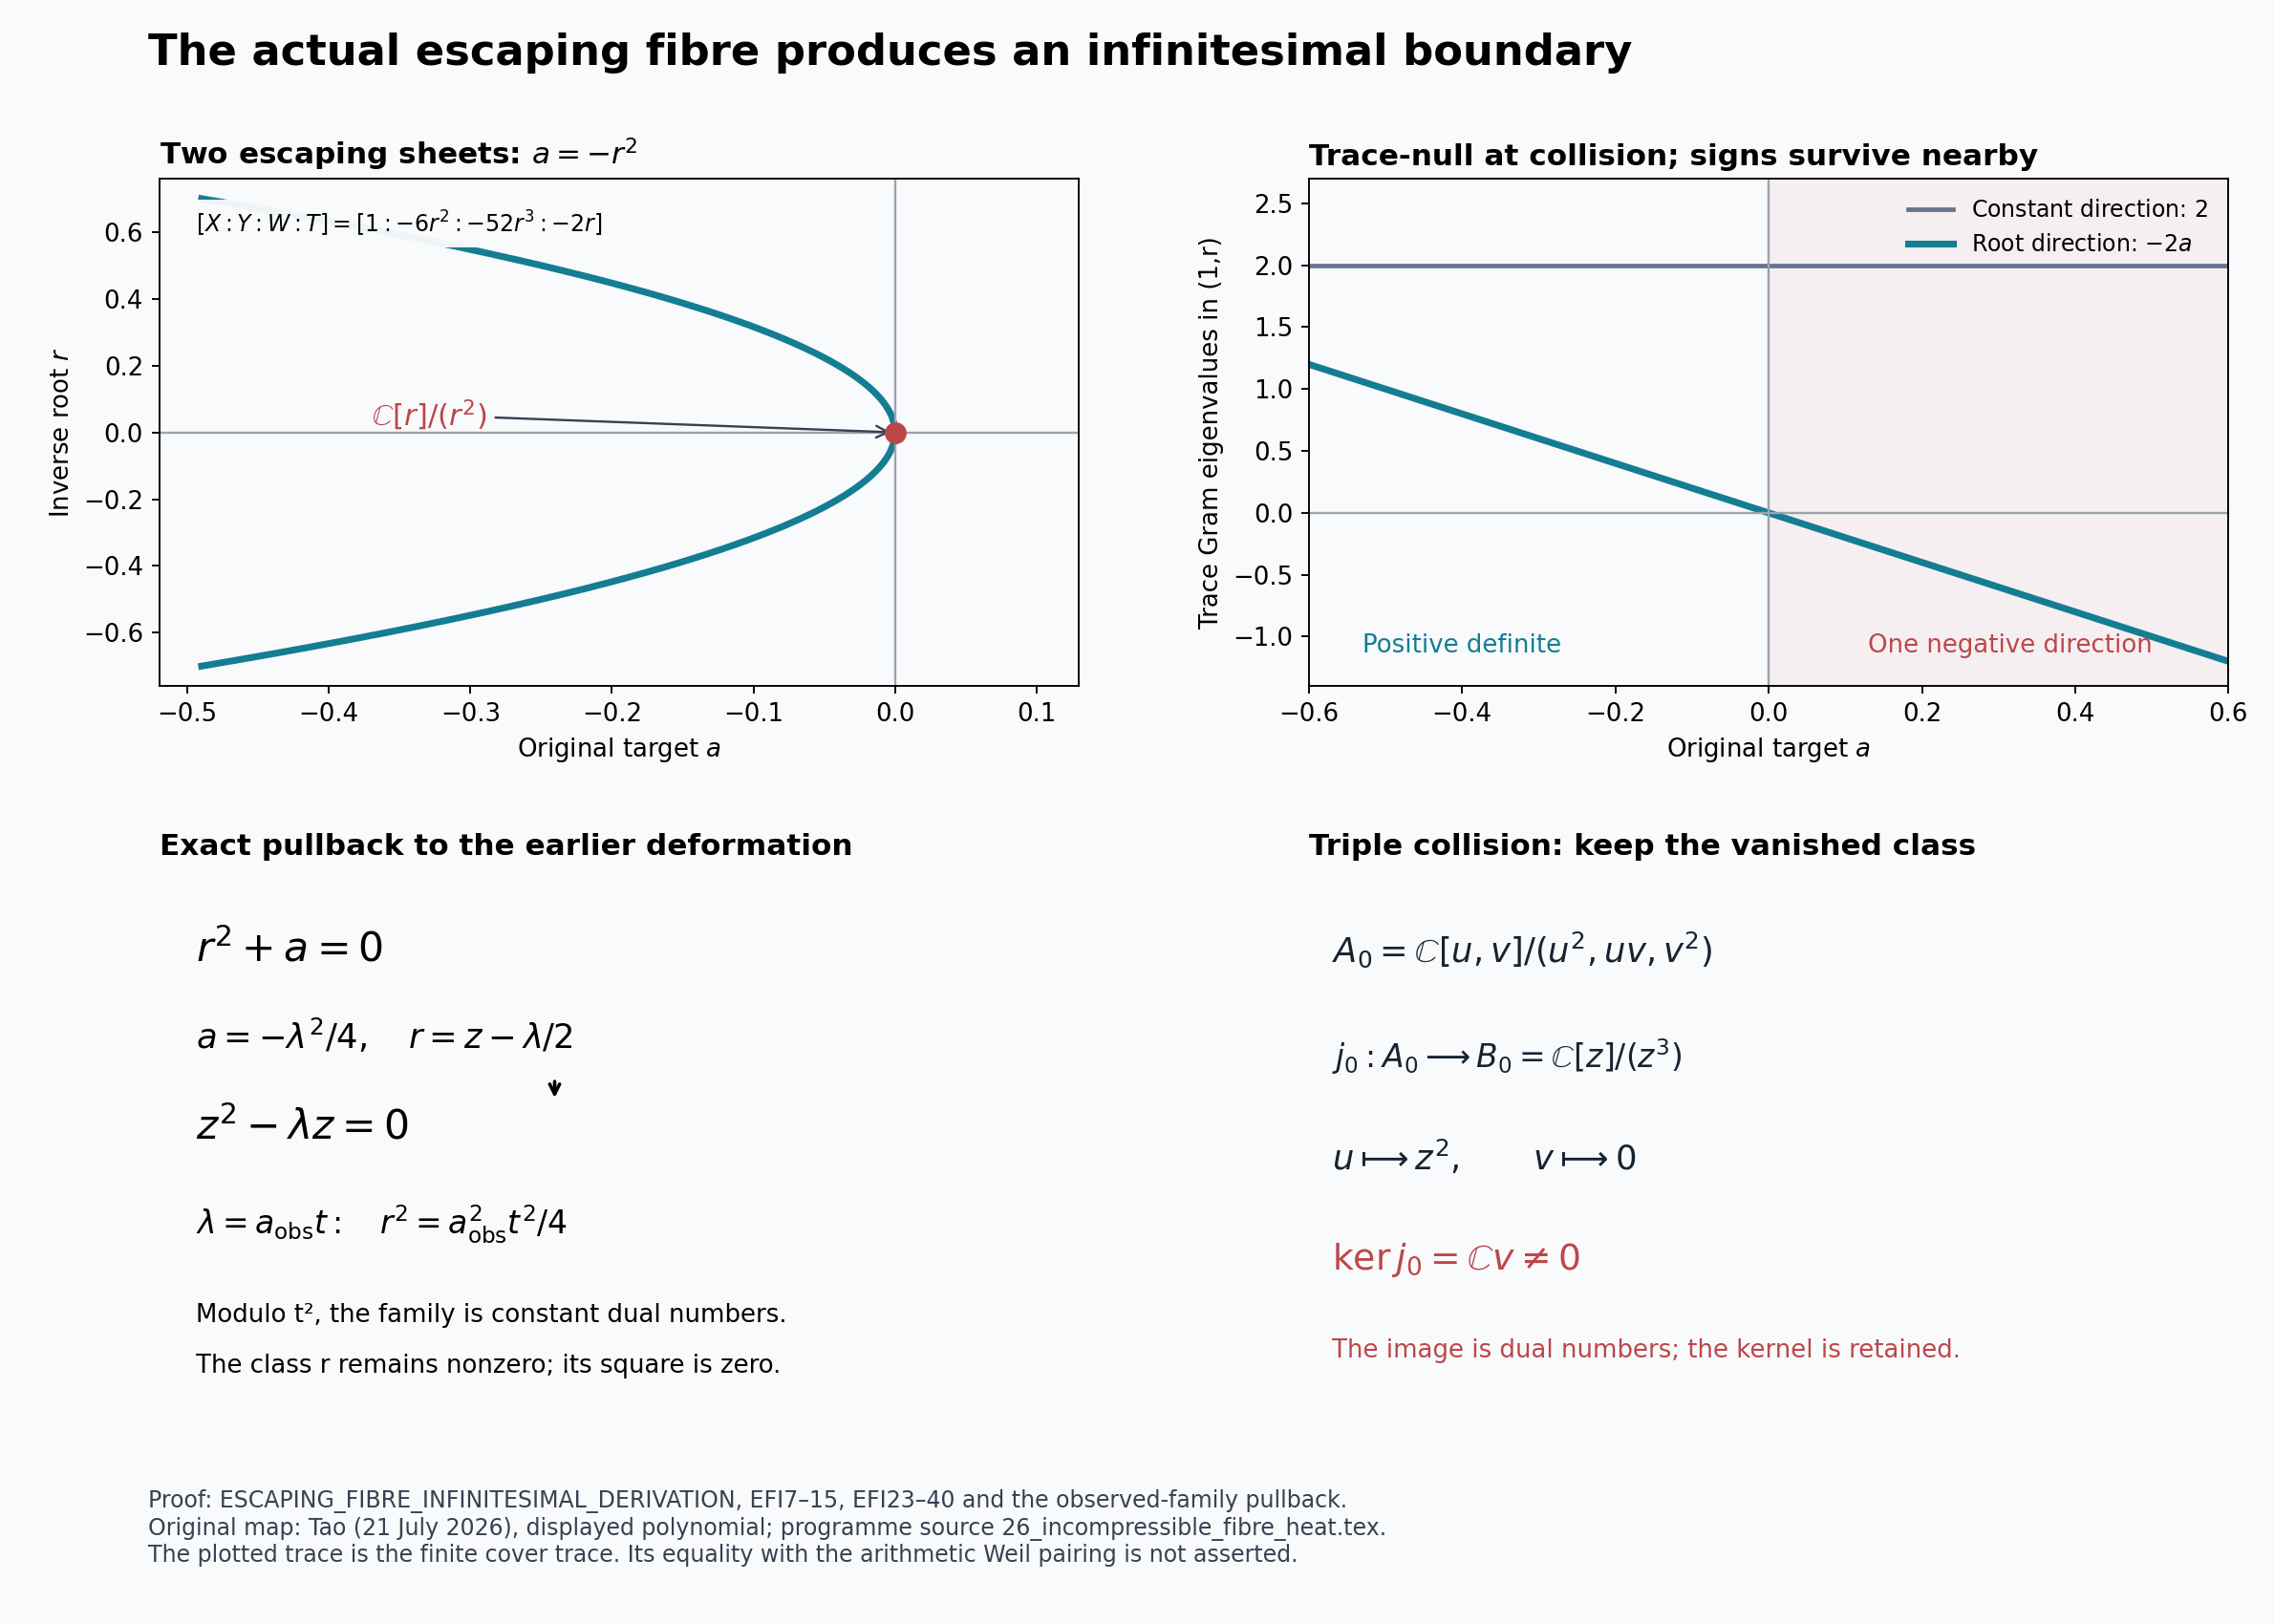
\includegraphics[keepaspectratio,alt={The exact cover a=-r² and finite trace eigenvalues; the observed-family pullback retains the collision generator. The triple graph map retains its kernel. Proof: EFI7--EFI15, EFI23--EFI40, EFI51--EFI68.}]{figures/25_escaping_trace.png}}
\caption{The exact cover a=-r² and finite trace eigenvalues; the
observed-family pullback retains the collision generator. The triple
graph map retains its kernel. Proof: EFI7--EFI15, EFI23--EFI40,
EFI51--EFI68.}
\end{figure}

\end{document}
